\title{PLUTO simulation and imaging procedures}
\author{Jonathan}
\date{\today}
\documentclass[12pt]{article}

\usepackage{graphicx}


\begin{document}
\maketitle

\noindent This document outlines the general processes required to simulate an astrophysical jet using PLUTO, and provides general instructions on imaging your simulation using python.\\
\newline
Note that it is assumed that the user has python 2.7 installed, as the pyPLUTO python module that comes with PLUTO does not work in python 3.
\section{PLUTO}

PLUTO is a user-friendly finite-volume, shock-capturing code that was written to integrate a set of conservation laws such as hydrodynamical equations. There are four inbuilt physics modules (C++?) allowing for hydrodynamical, magnetohydrodynamical, special relativistic hydrodynamical, and relativistic magnetohydrodynamical physics to be investigated.\\
\\
The code requires 4 files to run: init.c, definitions.h, pluto.ini and an appropriate makefile for your OS. The following sections summarise the role of each of these files, and give a brief how-to on setting up your own simulation with an emphasis on producing astrophysical jets. The latter sections discuss imaging your simulation using python. A more in-depth guide to PLTUO can be found at http://plutocode.ph.unito.it/files/userguide.pdf.

\subsection{Simulation set up}

The three important files that govern the behaviour of your simulation are the definitions.h, pluto.ini and init.c files. These files define the physics, and resolution of your simulation, the values of your input parameters (eg, Mach numbers, densities and pressures), temporal parameters such as how often results are printed to file, or the simulation length, and the time dependent boundary conditions.

\subsubsection{Definitions.h}
The definitions.h file is divided into 5 blocks, and sets the physics (eg, HD, MHD), geometry, Rieman solver and timestepper, number of user defined parameters and output of warning messages. The first three blocks of the definitions.h file can be configured easily by running the setup.py script.

- number of user defined parameters in the third block must match the value of USER$\_$DEF$\_$PARAMETERS in the first block.

- the geometry and body force selection must match the coding of your simulation in the init.c file

- max number of tracers accepted when running setup.py is 8, any more and you will need to manually edit the definitions.h file. Also any more than 8 and you won't be able to look at all of the parameters using the GUI as it is not optimized more >8 tracers.

\subsubsection{pluto.ini}
“pluto.ini (sets the number of grid zones, Riemann solver, output frequency, etc.),”
Selecting your grid
spherical coordinates\\
\\
The [Grid] section enables for resolution customisation of the simulation grid space. This is useful as finer grid spacings are required in some important areas of jet simulations. For example, in areas around the jet-environment boundary, a higher resolution grid is needed to be able to resolve turbulence. This is vitally important as turbulence plays a large role in momentum transfer from jets, causing differing morphologies (e.g. Perucho DATE). \\
the simulation grid is composed of 'grid patches'. Each grid patch may differ in:- 
\begin{itemize}
\item Size
\item Number of cells
\item Size of the cells comprising the patch; or
\item How the cells are distributed over the patch
\end{itemize}
For example, figure 1 below shows a 2D grid space extending out to x = 12.  There are 2 patches (as indicated by the shading). Patch 1 is 0 $\leq x < 6$ and contains 6 cells in x. Patch 2 is 6 $\leq x <$ 12 and contains half the amount of cells 3 cells. This is useful if finer resolution is needed for 'what is going on' below x = 6, and not required at lengths larger than that, and therefore the computation time benefits from the smaller grid.


The y direction is uniform - meaning that there is only 1 patch in the y direction.


The spacing of the cells in the $\hat{y}$ direction is larger for 5 < x <= 9
\begin{figure}[h]
	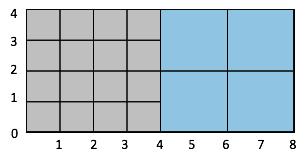
\includegraphics[width=8cm]{gridspaces}
	\centering
	\caption{Grid with even spacing in $\hat{y}$, but two patches with different spacings in $\hat{x}$}
\end{figure}


Write about tmax and dt
Write about output frequency
\subsubsection{init.c}
Setting up an environment
boundary condition\\
\\
the init.c file sets up the boundary conditions (which are a function of time) of your simulation grid. The manipulation of the lower (x,y) boundary (or lower (r) boundary on a spherical grid) to include an inflow of conserved simulation quantities is used to simulate a fluid jet. These quantities can also be user defined (see definitions.h section).

need to put in the actual code here and talk about it. show code for
'initial conditions'
'user defined boundary conditions'
'gravity bit at the end'

\subsection{Viewing your data}
[Viewing the simulation]
There is an pre-coded GUI that uses the pyPLUTO python module to display 2D images, or slices of your simulation output. However, the resolution at which the GUI displays the data is less than the actual resolution of the simulation (this is usually the case when the grid spacing is low enough to resolve turbulence). It is much easier to get a better looking image by importing the pyPLUTO module into pluto yourself, and manually extracting the data from the pyPLUTO object. This section outlines how to use the pyPLUTO code, how to create images, and a small introduction to making movies of your simulations.

'the things you can do by doing that, eg how to make surface brightness plots etc'

Nondimensionalization of the simulation
-length scales

Making a movie


\end{document}